\chapter{MATERYAL VE YÖNTEM}

Basit iki terimle \acrfull{OBEB} ve \acrfull{OKEK} kısaltmaları anlatabiliriz. İster kısaltmasını \acrshort{OBEB}, isterseniz de uzun açılımını \acrlong{OKEK} yazdırabilirsiniz. Bunu yapabilmek için dosyanın başında terimleri tanımlamanız gereklidir. İsterseniz matematik terimlerini de, örneğin \acrshort{pi} böyle tanımlayabilirsiniz. Uzun uzun \acrfull{pi} yazmanız gerekmez. 

Teorem yazmak isterseniz:
\begin{theorem}[Öklid]
 İki noktadan bir ve yalnız bir doğru geçer.
\end{theorem}

İspat yazmak isterseniz:
\begin{ispat}[Tezin en önemli ispatı]
x=10
\end{ispat}
\lipsum[1-2]
\begin{figure}[h]
\centering
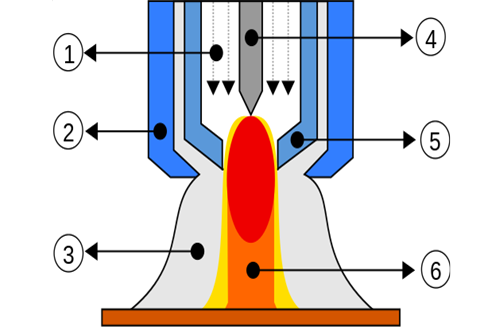
\includegraphics[width=\textwidth]{gorseller/ptaTorc}
\caption{PTA Torç}\label{fig:PtaTorc1}
\end{figure}
\lipsum[1-2]
\begin{table}
\centering
\caption{Deneme Tablosu.}\label{tab:den1}
\begin{tabular}{|l|l|l|}
\hline
sıra   & sayı   & toplam \\ \hline
1      & 2      & 3      \\ \hline
Kelime & deneme & son    \\ \hline
\end{tabular}
\end{table}


\section{Bulgular ve Tartışma Birinci Derece Başlık}
\lipsum[1-2]
\begin{figure}[h]
\centering
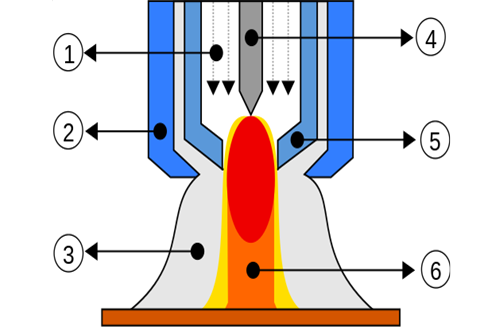
\includegraphics[width=\textwidth]{gorseller/ptaTorc}
\caption{PTA Torç}\label{fig:PtaTorc1}
\end{figure}
\lipsum[1-2]
\begin{table}
\centering
\caption{Deneme Tablosu.}\label{tab:den1}
\begin{tabular}{|l|l|l|}
\hline
sıra   & sayı   & toplam \\ \hline
1      & 2      & 3      \\ \hline
Kelime & deneme & son    \\ \hline
\end{tabular}
\end{table}
Teorem yazmak isterseniz:
\begin{theorem}[Öklid]
 İki noktadan bir ve yalnız bir doğru geçer.
\end{theorem}

İspat yazmak isterseniz:
\begin{ispat}[Tezin en önemli ispatı]
x=10
\end{ispat}

\subsection{Bulgular ve Tartışma ikinci derece başlık}
\lipsum[1-2]
\begin{figure}[h]
\centering
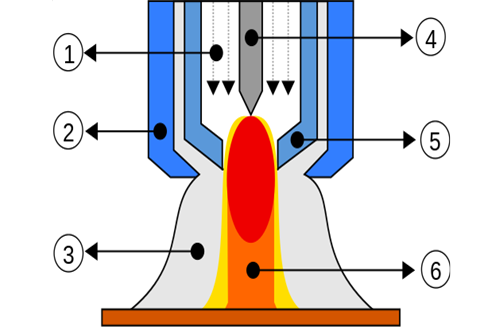
\includegraphics[width=\textwidth]{gorseller/ptaTorc}
\caption{PTA Torç}\label{fig:PtaTorc1}
\end{figure}
\lipsum[1-2]
\begin{table}
\centering
\caption{Deneme Tablosu.}\label{tab:den1}
\begin{tabular}{|l|l|l|}
\hline
sıra   & sayı   & toplam \\ \hline
1      & 2      & 3      \\ \hline
Kelime & deneme & son    \\ \hline
\end{tabular}
\end{table}

Teorem yazmak isterseniz:
\begin{theorem}[Öklid]
 İki noktadan bir ve yalnız bir doğru geçer.
\end{theorem}

İspat yazmak isterseniz:
\begin{ispat}[Tezin en önemli ispatı]
x=10
\end{ispat}

\subsubsection{Bulgular ve tartışma dördüncü derece başlık}
\lipsum[1-2]
\begin{figure}[h]
\centering
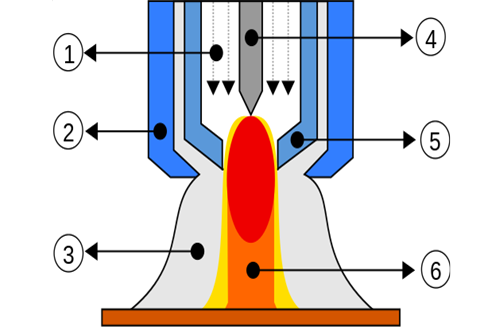
\includegraphics[width=\textwidth]{gorseller/ptaTorc}
\caption{PTA Torç}\label{fig:PtaTorc1}
\end{figure}
\lipsum[1-2]
\begin{table}
\centering
\caption{Deneme Tablosu.}\label{tab:den1}
\begin{tabular}{|l|l|l|}
\hline
sıra   & sayı   & toplam \\ \hline
1      & 2      & 3      \\ \hline
Kelime & deneme & son    \\ \hline
\end{tabular}
\end{table}

Teorem yazmak isterseniz:
\begin{theorem}[Öklid]
 İki noktadan bir ve yalnız bir doğru geçer.
\end{theorem}

İspat yazmak isterseniz:
\begin{ispat}[Tezin en önemli ispatı]
x=10
\end{ispat}
Eğer metin içinde \(\lim_{x \to \infty} \exp(-x) = 0\) ya da ortalayabilir
\begin{displaymath}
\cos (2\theta) = \cos^2 \theta - \sin^2 \theta
\end{displaymath}
isterseniz de numaralı denklem yazabilirsiniz.

\begin{equation}
\frac{\mathrm d}{\mathrm d x} \left( k g(x) \right)
\end{equation}
\subsubsection{Kimya}
\ce{B4C} yazabilirsiniz. Ya da

\ce{CO2 + C -> 2CO}

Daha fazlası için mhchem paketine bakınız.
 
\section{Analiz}
Eğer metin içinde şekile referans vermek isterseniz Şekil\ref{fig:PtaTorc} yazarsınız. 

Kaynakça böyle verilebilir \parencite{celik_microstructure_2013} ya da iki yazarlı ise böyle verilebilir \parencite{gatto_plasma_2004} veya ikiden fazla ise böyle verilebilir.
\parencite{celik_effects_2011}

Kaynakça listesi için daha çok referans verilmek istenirse \parencite{yazdi_microstructure_2015, keehan_influence_2006, guo_microstructure_2014}, \parencite{kim_variation_2013}, bir başkası \parencite{xibao_metallurgical_2005},  ya da başkası \parencite{jin_effect_1997} kullanılabilir.
